\section{Shape Matching}
\label{sec:shapeMatching}
Since shape detection performs on multiple scales and shapes are extracted for local regions only, a heuristic is needed to determine if shapes from different nodes belong to the same structure. While on a low level-of-detail, a wall is contained by a single octree node, on higher level, a node will only contain parts of the wall and mutliple nodes contain a primitive shape belonging to this wall. This section presents a set of matching functions to determine if two shapes are matching, e.g. originate from the same geometry. Only shapes of the same type can be matching.  Therefore it is not neccessary to define functions to match e.g. a plane shape with a cone shape, since the result will always be \verb|false|. 
\\
\\
As the primitive shapes are represented by only a handful of parameters, it is sufficient to determine the matching of these parameters.  Therefore, we firstly define elementary matching functions for floats, vectors, positions and axis. Since matching is an approximation of mathematical equality, each matching function's result is determined by comparing a computation result to a threshold $\epsilon$. If a matching function returns \verb|true|, the input values are considered to be matching. 

\begin{itemize}
	\item \textbf{Matching floats $f_1, f_2$}: 
		$$\frac{f_1}{f_2} \geq \epsilon, \textrm{ where } f_1 \leq f_2$$  
	\item \textbf{Matching vectors $v_1, v_2$}: 
		$$\frac{v_1}{|v_2|} \cdot \frac{v_2}{|v_2|} \geq \epsilon$$
	\item \textbf{Matching positions $p_1, p_2$}: 
		$$\sqrt{(p_1.x - p_2.x)^2 + (p_1.y - p2_y)^2 + (p1_z - p2_z)^2} \leq \epsilon$$
	\item \textbf{Matching axis $a_1, a_2$}: 
	\\
	An axis is defined by an start point and an endpoint. Let $p_{01},p_{02}$ be the start and end point of $a_1$ and $p_{12}, p_{12}$ the start and end point of $a_2$. Furthermore, let $v_1, v_2$ be the direction vectors of $a_1$ and $a_2$. The rays of the axis are denoted as $r_1 = p_{00} + sv_1$ and $r_2 = p_{10} + tv_2$. The closest distances for start and end point for each axis to the ray of the other axis are calculated. From those for values, the largest value $d$ is used for decision making. The matching decision is composed as follows: 
		$$\frac{v_1}{|v_2|} \cdot \frac{v_2}{|v_2|} \geq \epsilon_1 \land d \leq \epsilon_2$$
\end{itemize}


With the elementary matching functions defined, it is easy to define matching functions for two primitive shapes based on the elementary matching functions:

\begin{itemize}
\item \textbf{Matching plane shapes}: 
A plane shape contains to a quad that encloses all support points. For distance computation, the plane is used, rather than the quad. 
For each corner of each quad, the distance to the other plane is calculated. From those eight values the largest distance $d$ is chosen. Two plane shapes are matching, if the direction vectors are matching in retrospect to a threshold value $\epsilon_1$ and $d$ is smaller than or equal to a threshold value $\epsilon_2$.
\item \textbf{Matching cylinder shapes}: 
Cylinder consist of an axis and a radius. Two cylinder shapes are matching if both radii and both axes are matching. 
\item \textbf{Matching cone shapes}:
Cones consist of an axis and apex and an opening angle. Two cone shapes are matching if the axes, apexes and opening angles are matching. 
\item \textbf{Matching sphere shapes}: 
Two sphere shapes are matching, if the center positions and the radii are matching. 
\item \textbf{Matching torus shapes}: 
A torus consists of a center position, an axis and a major and minor radius. Two torus shapes are matching if the center position, axes, major radii and minor radii are matching. 
\end{itemize}

The matching result heavily depends on the chosen threshold values. Table \ref{tab:matchingThresholds} shows the $\epsilon$ values for primitive shape matching used for this thesis. Plane matching uses a custom heuristic that is not depicted in the table. For this heuristic, $\epsilon_2 = 0.05$ is chosen. Note that matching floats is a relative measure, whereas matching positions and axes uses world space distances as threshold. Matching vectors uses the angle between the two vectors to calculate a matching. 

\begin{table}
\centering
\begin{tabular}{ r | r }
	Matching	& threshold values \\
	\hline
  Floats 		& $\epsilon = 0.99$ \\
	Vectors 	& $\epsilon = 0.95$ \\
  Positions & $\epsilon = 0.05$ \\ 
	Axis 			& $\epsilon_2 = 0.05$, $\epsilon_1 = 0.95$ \\  

\end{tabular}
\caption{The different threshold values for parameter matching.}
\label{tab:matchingThresholds}
\end{table}


\section{Shape Clustering}

For the purpose of usability a small shape is not sufficient. To determine the global extent of a primitive shape, more information is needed. Section \ref{sec:shapeMatching} describes a set of heuristics to determine if two primitive shapes have the same origin. These heuristics are used in the section as well in order to create larger representations of a primitive shape. 
\textit{Shape Clustering} aim to find matching primitive shapes for a base shape and build a larger coherent cluster over multiple level-of-details. 
In order to find matching shapes, the octree is consulted and all shapes are collected that match the base shape. Already, the cluster consists of shapes that have the same geometry as origin. For finite shapes, this step is sufficient enough to create a valid cluster. However, for infinite shapes, such as planes further filtering is needed in order to create a coherent shape cluster. Figure \ref{fig:cuboids} shows the case of two cuboids, whose front face share a plane. However, by only using the matching functions to create a cluster, both front faces are packed into the cluster, even tough there is a visible gap between them.

\begin{figure}
	\centering
	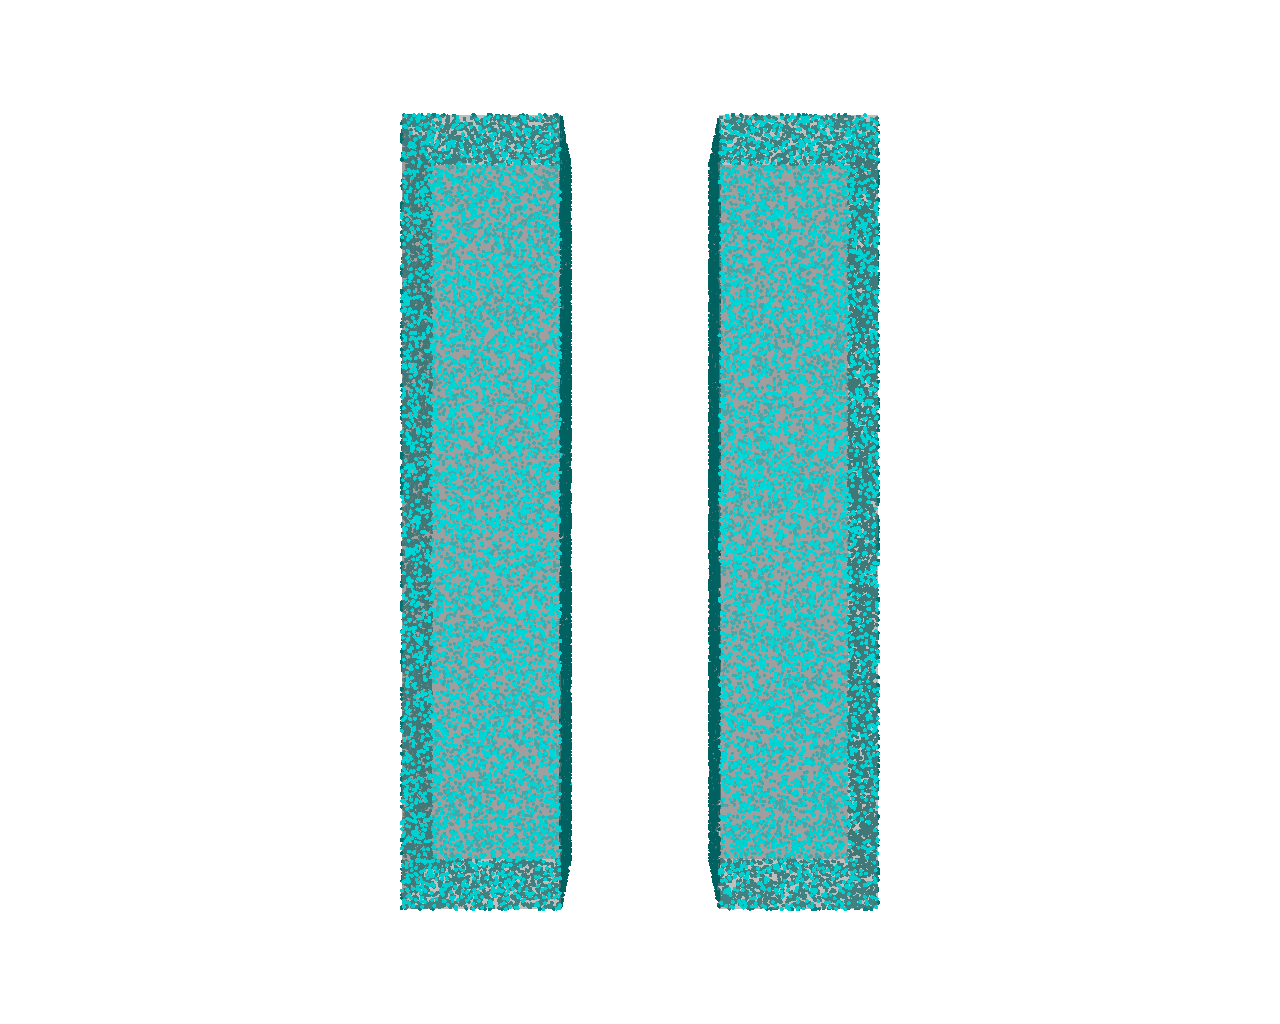
\includegraphics[width=0.8\textwidth]{Shape_Detection/cuboids.png}
	\caption{A generic point cloud of two cuboids. The detected planes are rendered in grey.}
	\label{fig:cuboids}
\end{figure}

A cluster of shapes can be seen as an $\epsilon$-connected component such as in graph theory. From all shapes that match the base shape, a complete graph is created. The set of shapes creates the set of vertices. In a complete graph, an edge exists for any pair of vertices. The weight of an edge is determined by the closest distance between the two shapes. A cluster is created by growing a region in a graph, adding only vertices that connect to the current region via an edge, whose weight is smaller than $\epsilon$. This creates a cluster of shapes, ensuring that the distance to the closest neighboring shape is at maximum $\epsilon$. 
\\
Figure \ref{fig:regionGrowingPlanes} shows an exemplary illustration on region growing for planes. The distance between two plane shapes is measured as the closest distance between the two bounding quads. The distances for cylinder and cone shapes are calculated differently. While for plane shape, the closest world space distance is used, matching cylinder and cone shapes use the distance between two start/end points. The matching heuristic already confirms that the shapes lie on the same axis and share a similar radius. Therefore, instead of a three-dimensional world distance, a one-dimensional distance along the axis is sufficient to build a shape cluster. Figure \ref{fig:regionGrowingConeCylinder} showcases clusters for both, cylinder shapes and cone shapes. 

\begin{figure}
	\centering
	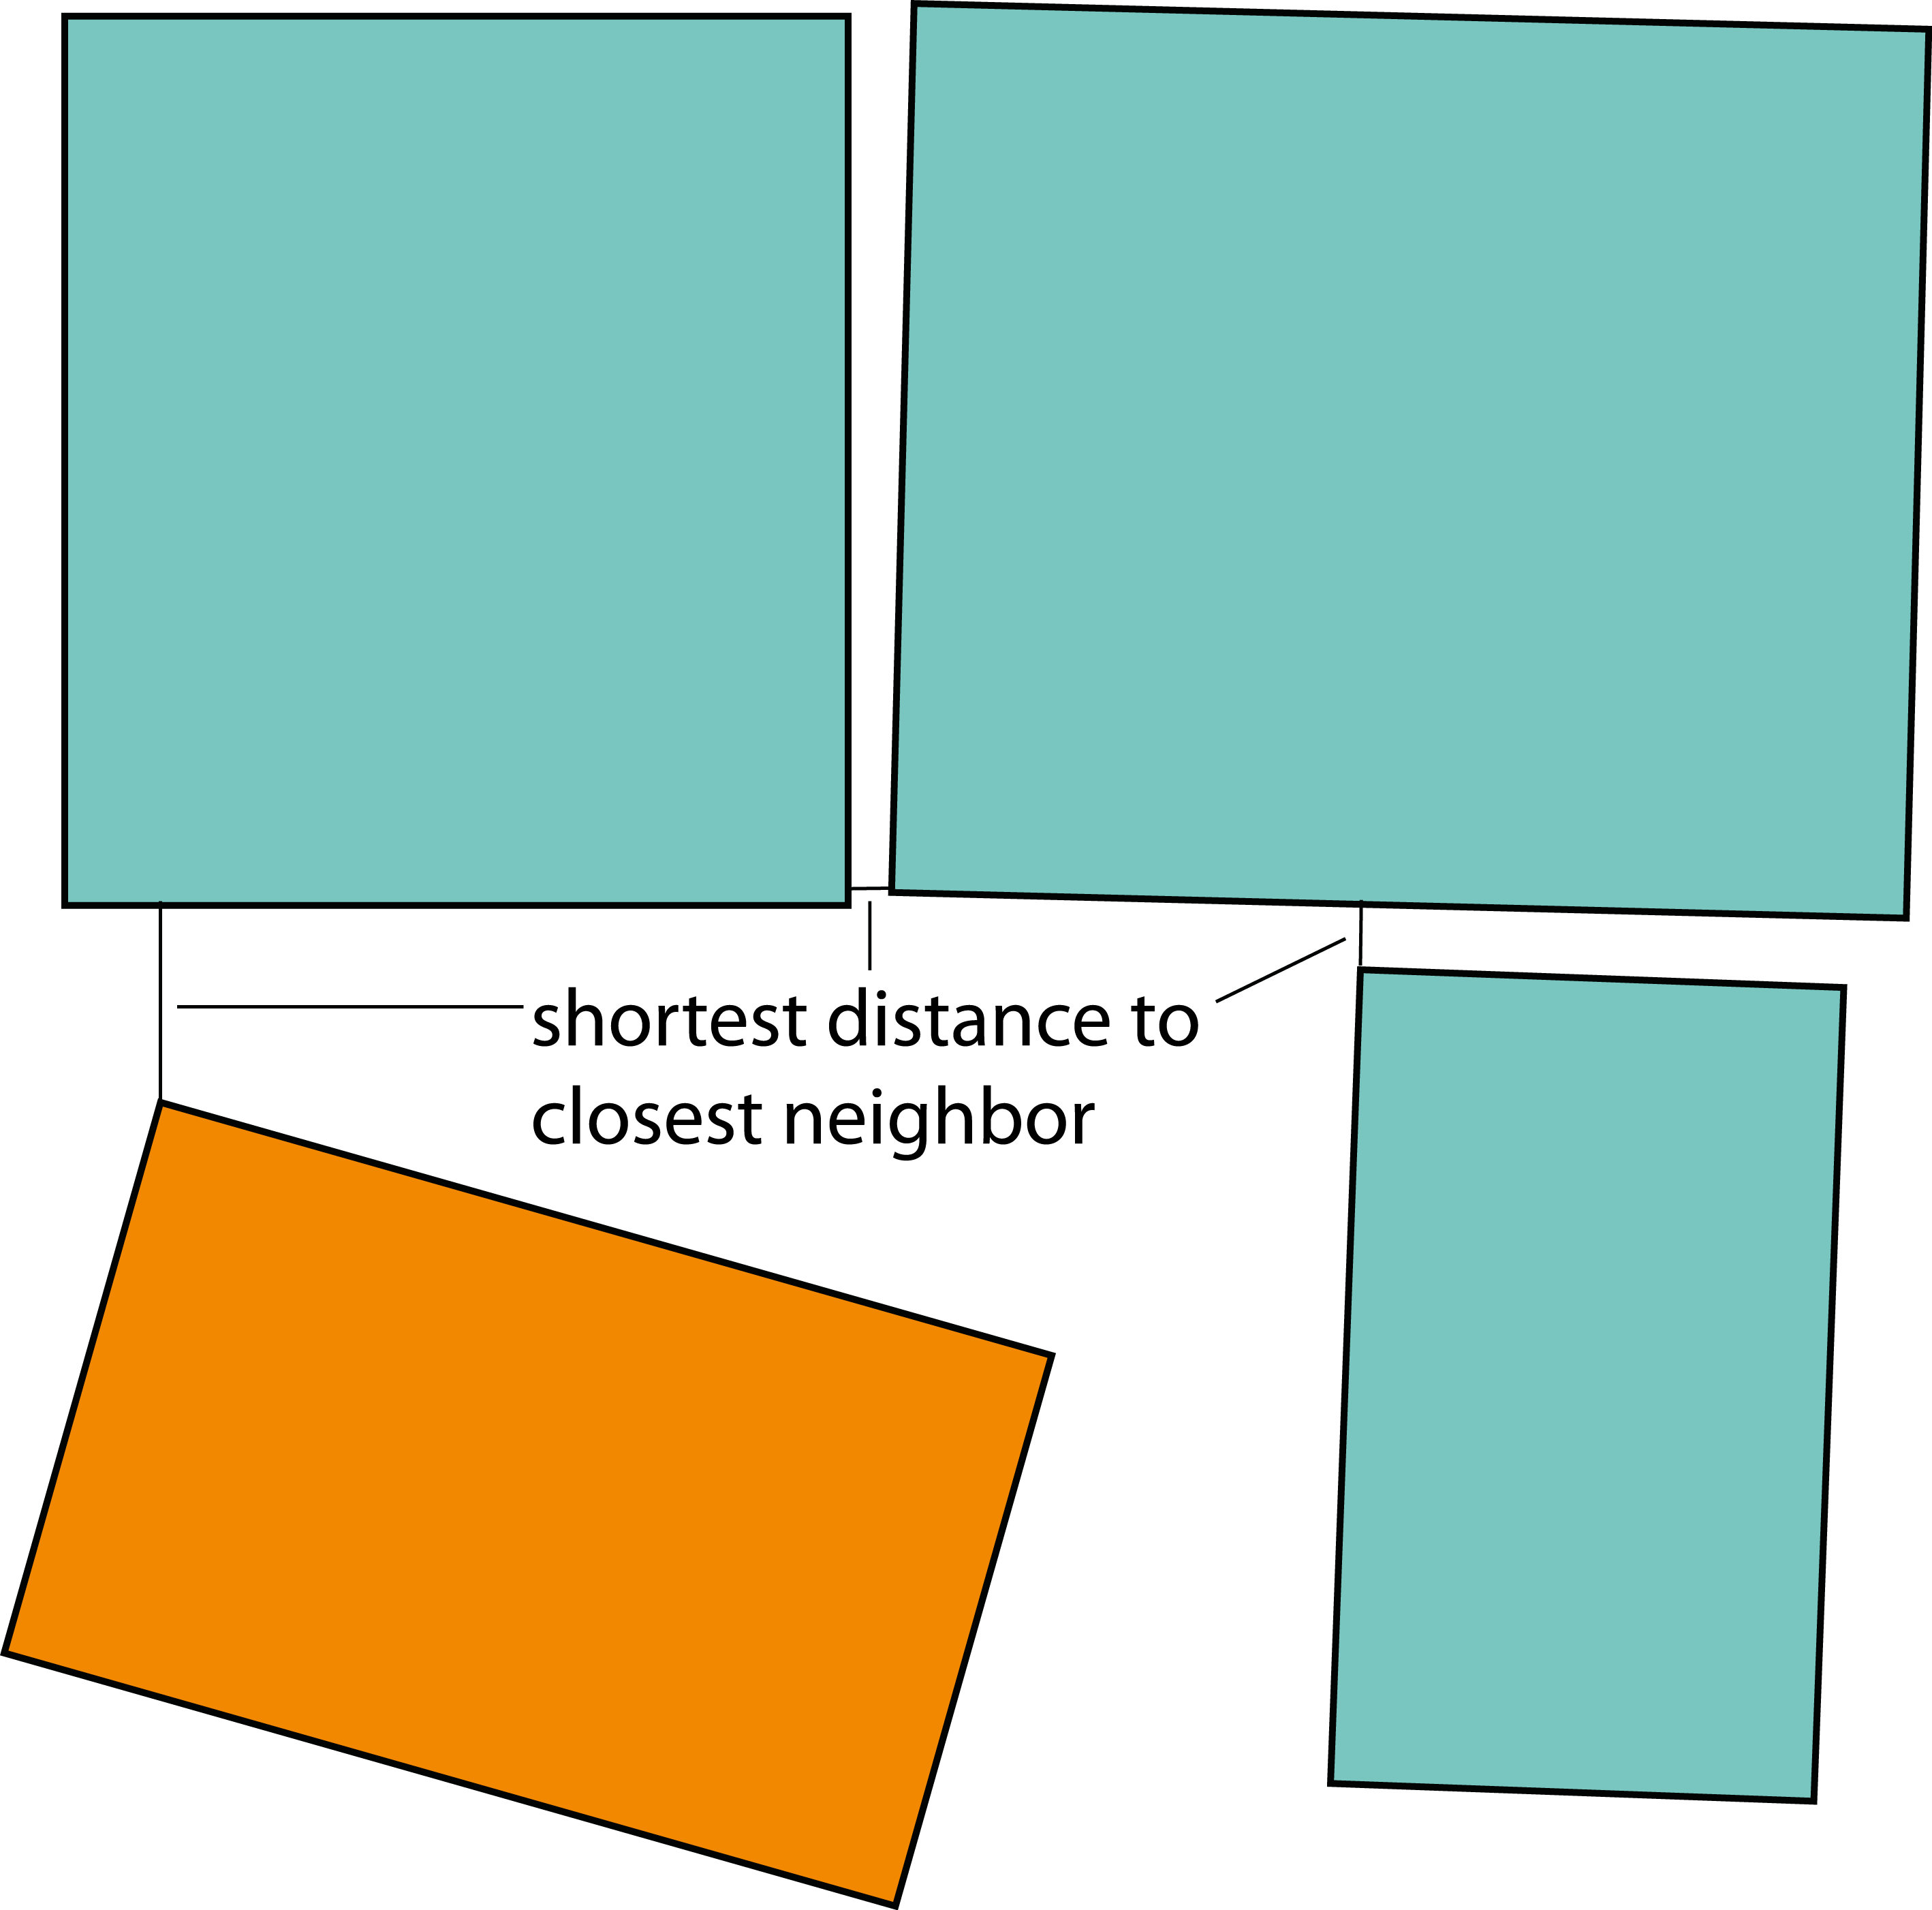
\includegraphics[width=0.5\textwidth]{Shape_Detection/regionGrowingPlanes.png}
	\caption{A cluster of plane shapes created by computing the $\epsilon$-connected component. Planes that belong to the cluster are colored in turquoise.}
	\label{fig:regionGrowingPlanes}
\end{figure}


\begin{figure}
\centering
\subcaptionbox{ \label{fig:regionGrowingCylinder}}{%
  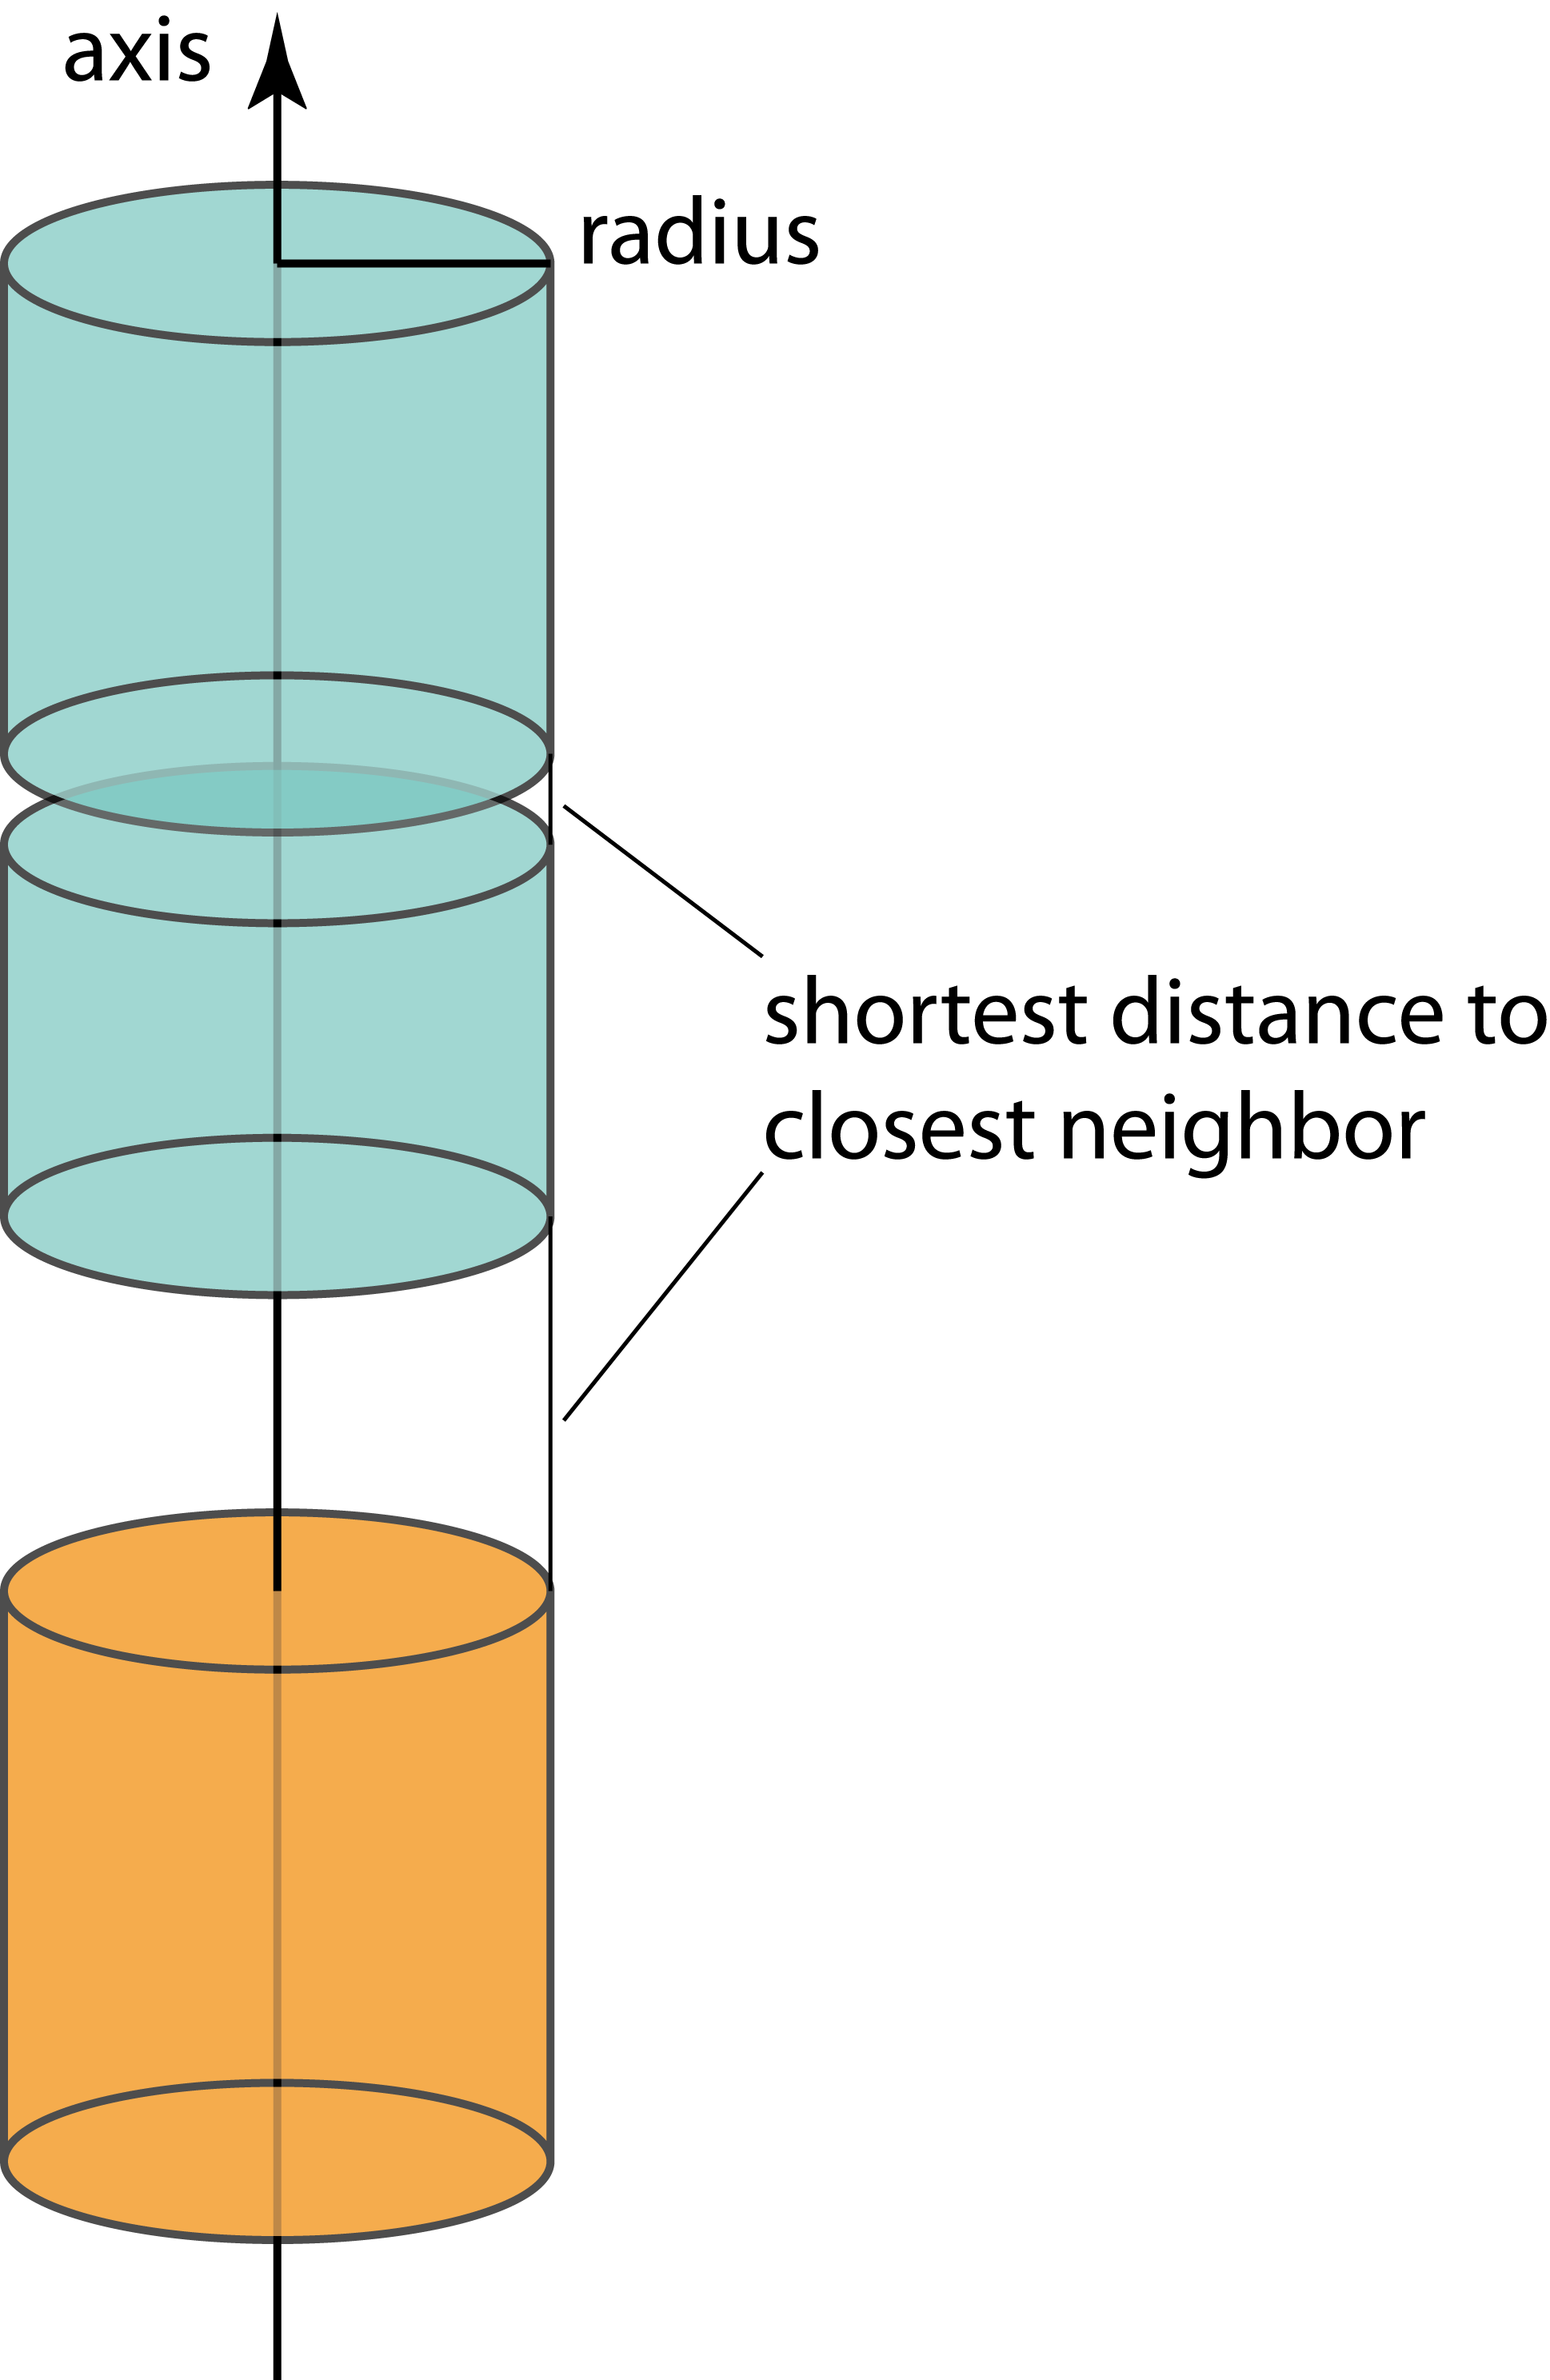
\includegraphics[width=0.3\textwidth]{Shape_Detection/regionGrowingCylinder.png}%7
  }
\subcaptionbox{ \label{fig:regionGrowingCone}}{%
  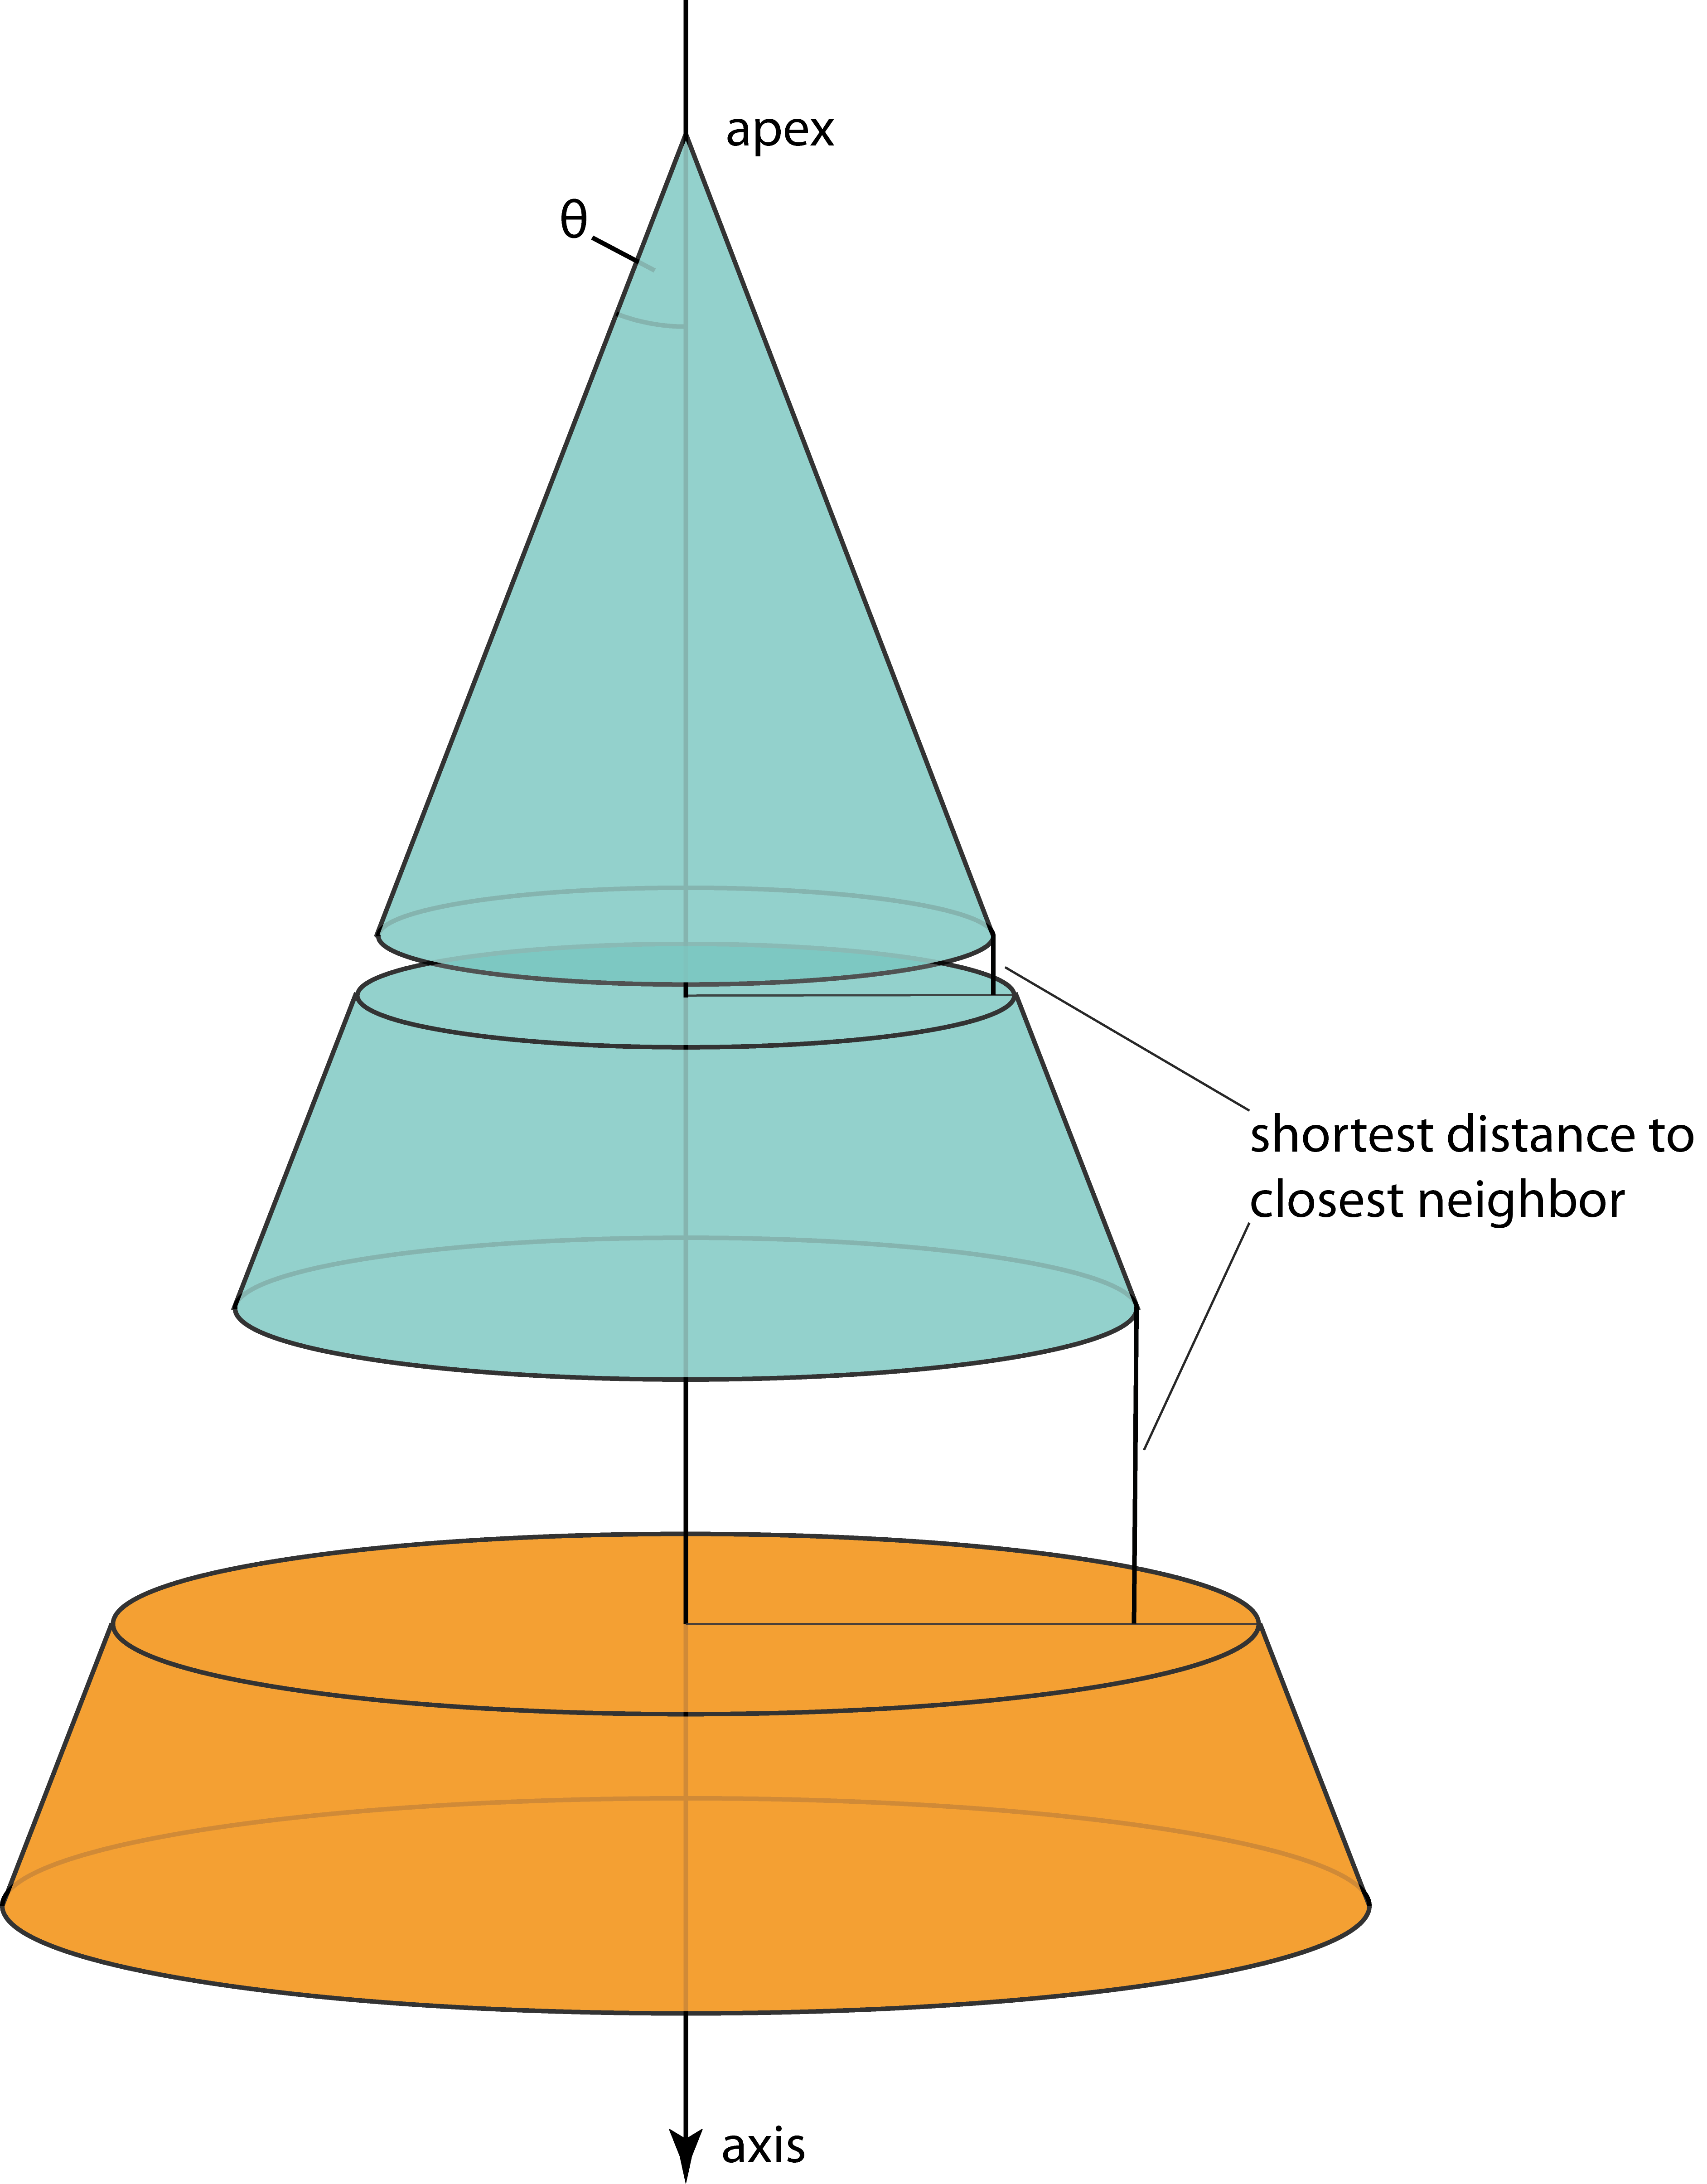
\includegraphics[width=0.5\textwidth]{Shape_Detection/regionGrowingCone.png}%
  }
	\caption{This figure shows a cylinder cluster and a cone cluster build from matching shapes. Shapes that belong to the cluster are colored in turqoise.}
	\label{fig:regionGrowingConeCylinder}
\end{figure}

The region growing component of the clustering heavily depends on the $\epsilon$ distance threshold. However, a proper distance threshold that mirrors the region's topology well is the density of an octree node as described in Section \ref{sec:shapeDetectionParameterSelection}. For this task we chose the density of the node of the base shape, more specific: $\epsilon = density \cdot 2.0$.